\documentclass[12pt,a4paper]{article}

% Include other packages here, before hyperref.
\usepackage{amsfonts}
\usepackage{amssymb}
\usepackage{amsmath}
\usepackage{amsthm}

\pdfoutput=1
\usepackage[pdftex]{graphicx}
\usepackage{times}

% If you comment hyperref and then uncomment it, you should delete
% egpaper.aux before re-running latex.  (Or just hit 'q' on the first latex
% run, let it finish, and you should be clear).
\usepackage[pagebackref=true,
            breaklinks=true,
            letterpaper=true,
            colorlinks,
            bookmarks=false]{hyperref}

\newtheorem{corollary}{Corollary}
\newtheorem{theorem}{Theorem}
\newtheorem{conjecture}[theorem]{Conjecture}
\newtheorem{definition}{Definition}
\newtheorem{lemma}{Lemma}
\newtheorem{remark}{Remark}
\newtheorem{proposition}{Proposition}
\newtheorem{fact}{Fact}

\def\1{\raisebox{2pt}{\rm{$\chi$}}}
\def\div{\mathop{\rm div}}
\def\argmax{\mathop{\rm arg\,max}}
\def\argmin{\mathop{\rm arg\,min}}
\def\at{\Bigr|}
\def\R{\mathbb{R}}
\def\S{\varGamma}
\def\x{\mathbf x}
\def\X{\mathbf X}
\def\y{\mathbf y}
\def\Y{\mathbf Y}
\def\O{\mathbf O}
\def\p{\mathbf p}
\def\e{\mathbf e}
\def\n{\mathbf n}


\begin{document}

\title{Geometry of Stereoscopic Filming and Displaying}
\author{Pau Gargallo}
\maketitle

\section{Formulas}
Shooting parameters
\begin{itemize}
 \item $f$ focal length
 \item $s_w, s_h$ the sensor width and height
 \item $b$ the interocular distance
 \item $C$ the convergence distance, i.e. distance to the stereoscopic window.
 \item $W$ width of the stereoscopic window. Can be computed from the other parameters. Assuming off-axis set up (using shift lenses or asymmetric camera frustum), we have
 \begin{equation}
  W_{offaxis} = \frac{s_w C}{f}
 \end{equation}
 If parallel cameras are used, then convergence is achieved by trimming the images which changes the width of the stereoscopic window. The width of the trim is equal to the interocular distance. Therefore the final width of the stereoscopic window will be
 \begin{equation}
  W_{trimmed} = \frac{s_w C}{f} - b
 \end{equation}
 \item $H$ the height of the stereoscopic window. This will depend of the type of cropping that is done. Without cropping we have
\begin{equation}
  H = \frac{s_h C}{f}
 \end{equation} 
 \item $Z$ is the depth of a given object
 \item $d$ is the disparity (or parallax) as a fraction of the window width, $W$.  By the Thales theorem we have
 \begin{equation}
  \frac{Z - C}{Z} = \frac{dW}{b}
 \end{equation}
 Which is equivalent to
 \begin{equation}
  d = \frac{b}{W} \frac{Z}{Z-C}
 \end{equation}
 and
 \begin{equation}
  Z = \frac{bC}{b - dW}
 \end{equation} 
\end{itemize}

\section{Viewing areas}
At a given depth plane, each camera sees a rectangular region of the plane.  We will describe this rectangle by its left, right, bottom and top coordinates. These coordinates are expressed in a reference centered at the middle point between the cameras' optical centers.

For the left cameras we have
\begin{equation}
 \begin{split}
  left &= \frac{1}{2} \left( Z \frac{b - W}{C} - b\right) \\
  right &= \frac{1}{2} \left( Z \frac{b + W}{C} - b\right) \\
  bottom &= -\frac{Z H}{2 C} \\
  top &= \frac{Z H}{2 C} ,
 \end{split}
\end{equation}
and for the right camera,
\begin{equation}
 \begin{split}
  left &= \frac{1}{2} \left( Z \frac{-b - W}{C} + b\right) \\
  right &= \frac{1}{2} \left( Z \frac{-b + W}{C} + b\right) \\
  bottom &= -\frac{Z H}{2 C} \\
  top &= \frac{Z H}{2 C} .
 \end{split}
\end{equation}



\section{CACA VELLA: Formulas}



\subsection{Filming}
\begin{figure}
 \begin{center}
  \includegraphics[width=0.9\textwidth]{stereo_projection.pdf}
 \end{center}
 \caption{Projection of a point into two cameras.  Or, equivalently, the perceived 3D point given the two images presented to the observer.}
\end{figure}


There are mainly 3 parameters that describe the internal geometry of a camera, and thus the way in which it captures images.  These are
\begin{itemize}
 \item the focal leghth of the camera, $f$,
 \item the width of the sensor, $w$
 \item and the position of the principal point, $\p$.
\end{itemize}
Usually, only the ratio between the focal length and the image width is relevant, and the principal point is at the origin.  In this discussion however, we have to take into account all 3 parameters since they are going to play and important role when displaying the images to the audience.

When filming in stereo, another parameter has to be controlled.  This is
\begin{itemize}
 \item the inter-camera distance or baseline, $b$.
\end{itemize}
Other parameters could also be taken into account to represent the relative position of cameras, but here, we are only going to consider parallel cameras with their optical center shifted on the x axis.  The reason is that other set ups yield to vertical disparity and should never be used without geometric correction.  A simplistic argument for this is that: since the images are going to be displayed in a single plane (the screen), they should also be captured in a single plane.  By placing the cameras in parallel position, we make their image planes coincide.


Let $b_c$ be the baseline or inter-occular distance of the cameras.  Let the optical centers of the cameras be
\begin{equation}
 \O^l = (-\frac{b_c}{2}, 0, 0)  \quad\quad  \O^r = (\frac{b_c}{2}, 0, 0)
\end{equation}
Let $f_c$ be the focal distance of the cameras and $w_c$ the width of the images expressed in the same units.  Let also $\p^l$ and $\p^r$ be the principal point of the cameras.


By Thales theorem we have
\begin{equation}
 \frac{p^l + w \x^l}{f} = \frac{\X_{xy} - \O^l_{xy}}{\X_z}
\end{equation}
This equation relates the 3D point $\X$ with its projection into the left image $\x^l$.  The same equation holds for the right image.


\begin{figure}
 \begin{center}
  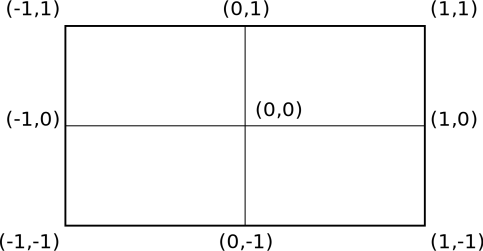
\includegraphics[width=0.7\textwidth]{image_coordinate.pdf}
 \end{center}
 \caption{The image coordinate system used in the equations.}
\end{figure}

\subsection{Displaying}
Ideally, one would like to display the images in the exact same set up that was used for filming.  If this was the case, the observer would view exactly what the cameras where seeing and the sensation of presence should be perfect, since there is no way for the observer to distinguish the images that are being shown from the ones that he should observe if she was actually there.

In practice, reproducing the exact same setup is not always possible.  In the following we are going to consider that the parameters such as the focal lenght $f$, the image width $w$, etc, are different when filming and when displaying, and we will analyse the geomtric effect iduced by this differences.



\end{document}

